\section*{Задание 1}
\subsection*{Постановка задачи}
Чем принципиально отличаются функции \texttt{cons}, \texttt{list}, \texttt{append}?\\
\indent Пусть \texttt{(setf lst1 '(a b))} \texttt{(setf lst2 '(c d))}\\
\indent Каковы результаты следующих выражений?

\begin{lstlisting}
(cons lst1 lst2)
(list lst1 lst2)
(append lst1 lst2)
\end{lstlisting}

\subsection*{Решение}
\begin{enumerate}
	\item \texttt{((A B) C D)}
	\item \texttt{((A B) (C D))}
	\item \texttt{(A B C D)}
\end{enumerate}

\section*{Задание №2}
\subsection*{Постановка задачи}
Каковы результаты вычисления следующих выражений?

\begin{lstlisting}
(reverse ())
(last ())
(reverse '(a))
(last '(a))
(reverse '((a b c)))
(last '((a b c)))
\end{lstlisting}


\subsection*{Решение}
\begin{enumerate}
	\item \texttt{Nil}
	\item \texttt{Nil}
	\item \texttt{(a)}
	\item \texttt{(a)}
	\item \texttt{((a b c))}
	\item \texttt{((a b c))}
\end{enumerate}

\section*{Задание №3}
\subsection*{Постановка задачи}
Написать, по крайней мере, два варианта функции, которая возвращает последний элемент своего списка-аргумента

\subsection*{Решение}
\begin{lstinputlisting}[label=third,caption=Решение задания №3, language=lisp, firstline=1, lastline=7]{../test.lisp}

\end{lstinputlisting}

\section*{Задание №4}
\subsection*{Постановка задачи}
Написать, по крайней мере, два варианта функции, которая возвращает свой список-аргумент без последнего элемента

\subsection*{Решение}
\begin{lstinputlisting}[label=third,caption=Решение задания №3, language=lisp, firstline=15, lastline=26]{../test.lisp}
	
\end{lstinputlisting}

\section*{Задание №5}
\subsection*{Постановка задачи}
Написать простой вариант игры в кости, в котором бросаются две правильные кости. Если сумма выпавших очков равна 7 или 11 --- выигрыш, если выпало $(1, 1)$ или $(6, 6)$ --- игрок получает право снова бросить кости, во всех остальных случаях ход переходит ко второму игроку, но запоминается сумма выпавших очков. Если второй игрок не выигрывает абсолютно, то выигрывает тот игрок, у которого больше очков. Результат игры и значения выпавших костей выводить на экран с помощью функции \texttt{print}.

\subsection*{Решение}
\begin{lstinputlisting}[label=third,caption=Решение задания №3, language=lisp, firstline=31, lastline=57]{../test.lisp}
	
\end{lstinputlisting}


\section*{Контрольные вопросы}
\textbf{Вопрос 1.} Синтаксическая форма и хранение программы в памяти.

\textbf{Ответ.}
В Lisp формы представления программы и обрабатываемых ею данных одинаковы – они представлены в виде S-выражений. Программы могут обрабатывать и преобразовывать другие программы или сами себя. В памяти программа представляется в виде бинарных узлов, так как она состоит из S-выражений.\newline

\textbf{Вопрос 2.} Трактовка элементов списка. 

\textbf{Ответ.}
Если отсутствует блокировка вычислений, то первый элемент списка трактуется как имя функции, а остальные элементы – как аргументы функции.\newline

\begin{figure}[H]
	\begin{center}
		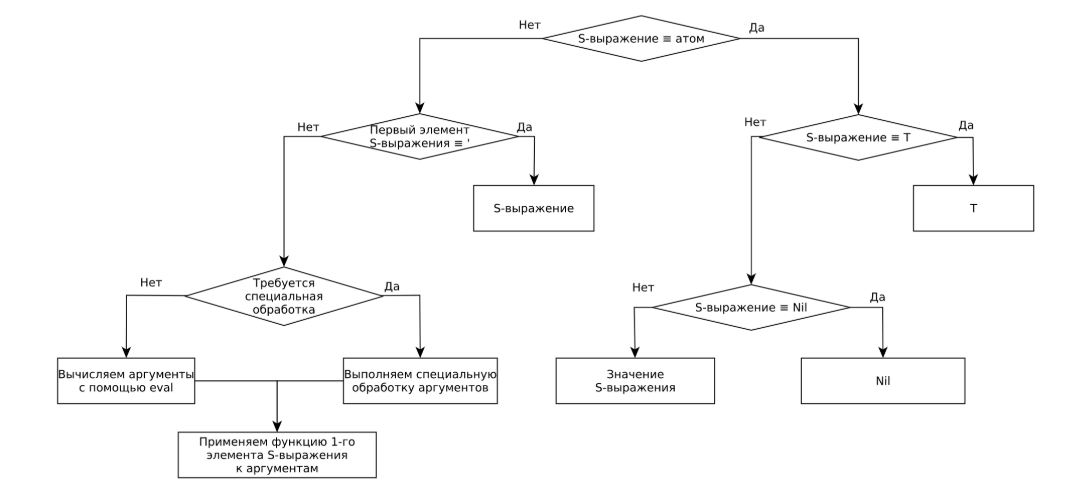
\includegraphics[scale=0.4]{img/eval.png}
	\end{center}
	\caption{Схема работы функции \textbf{eval}.}
	\label{img:eval}
\end{figure}

\textbf{Вопрос 3.} Порядок реализации программы.

\textbf{Ответ.}
Работа программы циклична: сначала программа ожидает ввода S-выражения, затем передает полученное S-выражение интерпретатору – функции eval, а в конце, после отработки функции eval, выводит последний полученный результат.\newline


\textbf{Вопрос 4.} Способы определения функции.

\textbf{Ответ.}
Функцию можно определить с помощью \textbf{defun} или \textbf{lambda.} 

(defun имя\_функции (список\_аргументов) тело\_функции)

(lambda (список\_аргументов) тело\_функции).
